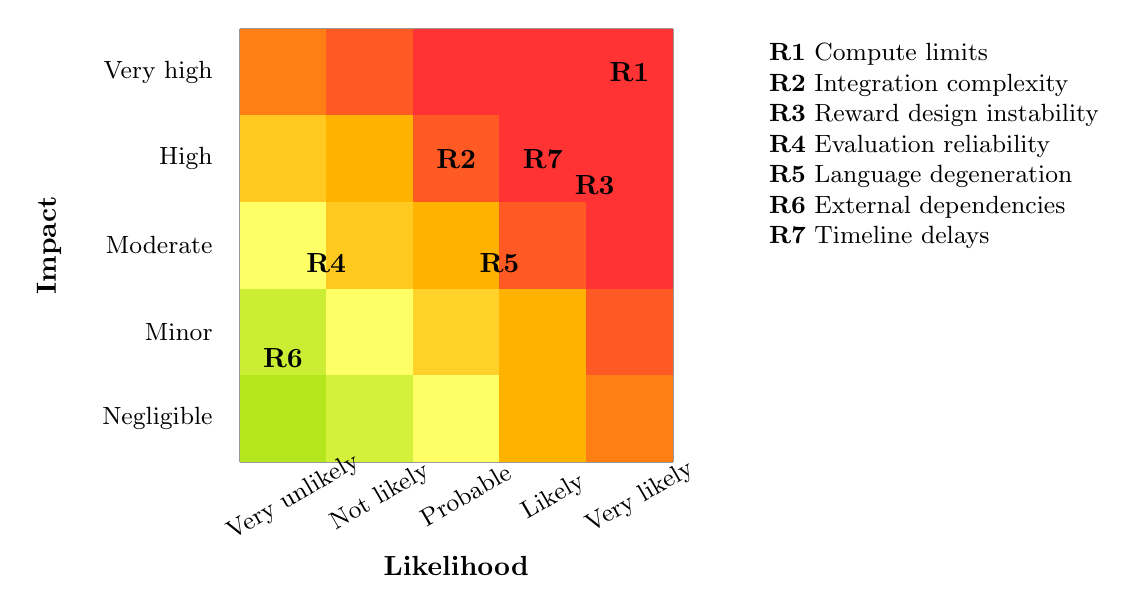
\begin{tikzpicture}[scale=1.1]

% Define improved colors based on the image
\definecolor{riskgreen}{RGB}{181,230,29}   % bright lime green
\definecolor{riskyellow}{RGB}{255,255,102} % vivid yellow
\definecolor{riskorange}{RGB}{255,178,0}   % strong orange
\definecolor{riskred}{RGB}{255,51,51}      % bright red

% Draw grid (5x5)
\foreach \x in {0,...,5} {
  \draw[gray!80, thick] (\x,0) -- (\x,5);
}
\foreach \y in {0,...,5} {
  \draw[gray!80, thick] (0,\y) -- (5,\y);
}

% Fill gradient cells (impact ↑, likelihood →)
\fill[riskgreen] (0,0) rectangle (1,1);
\fill[riskgreen!60!riskyellow] (1,0) rectangle (2,1);
\fill[riskyellow] (2,0) rectangle (3,1);
\fill[riskorange] (3,0) rectangle (4,1);
\fill[riskorange!60!riskred] (4,0) rectangle (5,1);

\fill[riskgreen!70!riskyellow] (0,1) rectangle (1,2);
\fill[riskyellow] (1,1) rectangle (2,2);
\fill[riskorange!60!riskyellow] (2,1) rectangle (3,2);
\fill[riskorange] (3,1) rectangle (4,2);
\fill[riskred!70!riskorange] (4,1) rectangle (5,2);

\fill[riskyellow] (0,2) rectangle (1,3);
\fill[riskorange!70!riskyellow] (1,2) rectangle (2,3);
\fill[riskorange] (2,2) rectangle (3,3);
\fill[riskred!70!riskorange] (3,2) rectangle (4,3);
\fill[riskred] (4,2) rectangle (5,3);

\fill[riskorange!70!riskyellow] (0,3) rectangle (1,4);
\fill[riskorange] (1,3) rectangle (2,4);
\fill[riskred!70!riskorange] (2,3) rectangle (3,4);
\fill[riskred] (3,3) rectangle (4,4);
\fill[riskred] (4,3) rectangle (5,4);

\fill[riskorange!60!riskred] (0,4) rectangle (1,5);
\fill[riskred!70!riskorange] (1,4) rectangle (2,5);
\fill[riskred] (2,4) rectangle (3,5);
\fill[riskred] (3,4) rectangle (4,5);
\fill[riskred] (4,4) rectangle (5,5);

% Axis labels (moved further out)
\node[rotate=90, font=\bfseries] at (-2.2,2.5) {Impact};
\node[font=\bfseries] at (2.5,-1.2) {Likelihood};

% Axis ticks
\foreach \y/\label in {0.5/{Negligible},1.5/{Minor},2.5/{Moderate},3.5/{High},4.5/{Very high}} {
  \node[left, font=\small] at (-0.2,\y) {\label};
}
\foreach \x/\label in {0.5/{Very unlikely},1.5/{Not likely},2.5/{Probable},3.5/{Likely},4.5/{Very likely}} {
  \node[below, font=\small, rotate=30] at (\x,-0.2) {\label};
}

% Risk positions
\node at (4.5,4.5) {\textbf{R1}};
\node at (2.5,3.5) {\textbf{R2}};
\node at (4.1,3.2) {\textbf{R3}};
\node at (1.0,2.3) {\textbf{R4}};
\node at (3.0,2.3) {\textbf{R5}};
\node at (0.5,1.2) {\textbf{R6}};
\node at (3.5,3.5) {\textbf{R7}};

% Legend
\node[align=left, font=\small, anchor=west] at (6,3.5) {
\textbf{R1} Compute limits \\
\textbf{R2} Integration complexity \\
\textbf{R3} Reward design instability \\
\textbf{R4} Evaluation reliability \\
\textbf{R5} Language degeneration \\
\textbf{R6} External dependencies \\
\textbf{R7} Timeline delays \\
};

\end{tikzpicture}